\chapter{Hajautustaulu}

\index{hajautustaulu}

\emph{Hajautustaulu} (\emph{hash table}) on tietorakenne,
joka pitää yllä alkioiden joukkoa.
Voimme tarkastaa,
kuuluuko tietty alkio joukkoon,
sekä lisätä ja poistaa alkioita.
Kuten matematiikassa, jokainen alkio
voi esiintyä enintään kerran joukossa.
Hajautustaulussa kaikki yllä mainitut
operaatiot toimivat tehokkaasti, mikä tekee siitä
kätevän työkalun algoritmien toteuttamisessa.

Tutustumme tässä luvussa ensin hajautustaulun
toimintaan ja sen tehokkuuteen
vaikuttaviin seikkoihin.
Tämän jälkeen käsittelemme Javan tietorakenteet
\texttt{HashSet} ja \texttt{HashMap},
jotka perustuvat hajautustauluun.
Lopuksi käymme läpi esimerkkejä tilanteista,
joissa voimme käyttää hajautustaulua
algoritmien suunnittelussa.

\section{Hajautustaulun toiminta}

\begin{figure}
\center
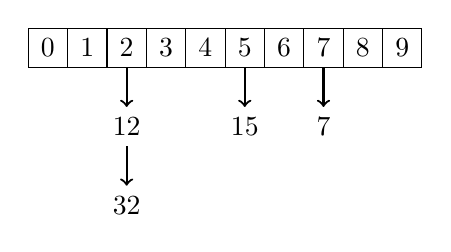
\begin{tikzpicture}[scale=0.5]
\draw (0,0) grid (10,1);
\foreach \x in {0,1,...,9} \node at (0.5+\x,0.5) {\x};
\draw[->,thick] (2.5,0) -- (2.5,-1);
\draw[->,thick] (5.5,0) -- (5.5,-1);
\draw[->,thick] (7.5,0) -- (7.5,-1);
\draw[->,thick] (2.5,-2) -- (2.5,-3);
\node at (2.5,-1.5) {$12$};
\node at (5.5,-1.5) {$15$};
\node at (7.5,-1.5) {$7$};
\node at (2.5,-3.5) {$32$};
\end{tikzpicture}
\caption{Hajautustaulu, joka vastaa joukkoa $\{7,12,15,32\}$.
Hajautusfunktiona on $f(x)=x \bmod 10$.}
\label{fig:hajtau}
\end{figure}

\index{hajautusfunktio}
\index{hajautusarvo}

Toteutamme hajautustaulun taulukkona,
jonka jokaisessa kohdassa on lista joukkoon kuuluvia alkioita.
Jotta voimme käyttää hajautustaulua,
tarvitsemme \emph{hajautusfunktion} (\emph{hash function}) $f$,
joka antaa \emph{hajautusarvon} (\emph{hash value})
$f(x)$ mille tahansa joukon alkiolle $x$.
Hajautusarvo on kokonaisluku väliltä
$0,1,\dots,N-1$, missä $N$ on hajautustaulun koko.
Tallennamme hajautustaulun kohdassa $k$ olevaan listaan
kaikki ne joukon alkiot, joiden hajautusarvo on $k$.

Kuvassa \ref{fig:hajtau} on esimerkkinä hajautustaulu,
jonka kokona on $N=10$.
Olemme tallentaneet hajautustauluun joukon $\{7,12,15,32\}$
käyttäen hajautusfunktiota $f(x)=x \bmod 10$.
Tämä tarkoittaa, että alkion $x$ hajautusarvo on sen jakojäännös $10$:llä
eli luvun viimeinen numero.
Esimerkiksi alkiot $12$ ja $32$ ovat kohdassa $2$,
koska niissä viimeinen numero on $2$,
ja alkiot $15$ ja $7$ ovat vastaavasti kohdissa $5$ ja $7$.
Kaikki muut hajautustaulun listat ovat tällä hetkellä tyhjiä.

Kun haluamme tarkastaa, onko joukossa alkiota $x$,
laskemme ensin sen hajautusarvon $f(x)$.
Tämän jälkeen käymme läpi kaikki kohdan $f(x)$
listassa olevat alkiot ja tarkastamme,
onko jokin niistä alkio $x$.
Vastaavasti kun haluamme lisätä alkion $x$ joukkoon
tai poistaa alkion $x$ joukosta,
teemme muutoksen kohdassa $f(x)$ olevaan listaan.
Jokaisen operaation aikavaativuus on $O(m)$,
missä $m$ on listan alkioiden määrä.
Hajautustaulu toimii siis tehokkaasti, jos jokainen
siinä oleva lista on lyhyt.

\subsection{Hajautusfunktio}

Hajautusfunktio $f(x)$ määrittää, mihin kohtaan hajautustaulua
alkio $x$ sijoitetaan.
Sen täytyy antaa jokaiselle mahdolliselle alkiolle
hajautusarvo eli kokonaisluku väliltä $0,1,\dots,N-1$,
missä $N$ on hajautustaulun koko.
Muilta osin meillä on periaatteessa vapaat kädet
hajautusfunktion suunnitteluun.
Mutta millainen olisi hyvä hajautusfunktio?

\begin{figure}
\center
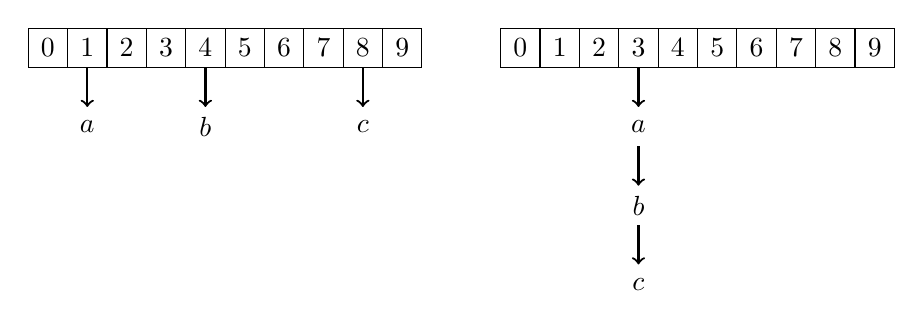
\begin{tikzpicture}[scale=0.5]
\begin{scope}
\draw (0,0) grid (10,1);
\foreach \x in {0,1,...,9} \node at (0.5+\x,0.5) {\x};
\draw[->,thick] (1.5,0) -- (1.5,-1);
\draw[->,thick] (4.5,0) -- (4.5,-1);
\draw[->,thick] (8.5,0) -- (8.5,-1);
\node at (1.5,-1.5) {$a$};
\node at (4.5,-1.5) {$b$};
\node at (8.5,-1.5) {$c$};
\end{scope}
\begin{scope}[xshift=12cm]
\draw (0,0) grid (10,1);
\foreach \x in {0,1,...,9} \node at (0.5+\x,0.5) {\x};
\draw[->,thick] (3.5,0) -- (3.5,-1);
\draw[->,thick] (3.5,-4) -- (3.5,-5);
\draw[->,thick] (3.5,-2) -- (3.5,-3);
\node at (3.5,-1.5) {$a$};
\node at (3.5,-3.5) {$b$};
\node at (3.5,-5.5) {$c$};
\end{scope}
\end{tikzpicture}
\caption{Kaksi hajautustaulua joukolle $\{a,b,c\}$.
Vasen tilanne on paras mahdollinen, oikea tilanne taas
huonoin mahdollinen.}
\label{fig:hajjak}
\end{figure}

Haluamme, että hajautusfunktio jakaa alkioita \emph{tasaisesti}
hajautustaulun eri puolille.
Jos onnistumme tässä, kaikki listat ovat lyhyitä ja
hajautustaulun operaatiot ovat tehokkaita.
Kuva \ref{fig:hajjak} näyttää kaksi hajautustaulua, jotka vastaavat
joukkoa $\{a,b,c\}$ kahdella eri hajautusfunktiolla.
Vasemmassa taulussa hajautus on onnistunut täydellisesti
ja jokainen alkio on omassa listassaan.
Oikeassa taulussa taas kaikki alkiot ovat joutuneet samaan
listaan eikä hajautuksesta ole mitään hyötyä.
Tavoitteemme on saada aikaan hajautusfunktio,
jonka toiminta on lähempänä vasenta tilannetta.

Jos hajautettavat alkiot ovat kokonaislukuja,
suoraviivainen hajautusfunktio on $f(x)=x \bmod N$,
missä "mod" on modulo eli jakojäännös,
joka muuttaa luvun välille $0 \dots N-1$.
Tämä on helposti toteutettava ja yleensä hyvin toimiva hajautusfunktio.
Entä jos alkiot ovat jotain muuta tyyppiä kuin kokonaislukuja?
Tällöin meidän täytyy päättää ensin jokin järkevä tapa,
kuinka muutamme alkion kokonaisluvuksi,
minkä jälkeen voimme jälleen ottaa jakojäännöksen $N$:llä.

Tarkastellaan esimerkkinä tilannetta, jossa haluamme hajauttaa merkkijonoja
eli mei\-dän täytyy löytää keino muuttaa merkkijono kokonaisluvuksi.
Oletamme, että merkkijonossa on $k$ merkkiä,
joiden merkkikoodit ovat $c_0,c_1,\dots,c_{k-1}$.
Esimerkiksi jos merkkijono on \texttt{testi},
merkkikoodit\footnote{Käytämme tässä merkkien ASCII-koodeja.
Esimerkiksi Javassa \texttt{char}-merkin \texttt{c} koodin saa
selville kirjoittamalla \texttt{(int)c}, eli esimerkiksi
\texttt{(int)'t'} on 116.} ovat $c_0=116$, $c_1=101$, $c_2=115$,
$c_3=116$ ja $c_4=105$.
Yksi tapa muuttaa merkkijono kokonaisluvuksi
on laskea merkkikoodien summa
\[ c_0 + c_1 + \dots + c_{k-1},\]
jolloin merkkijonoa \texttt{testi} vastaa kokonaisluku
\[116+101+115+116+105=553.\]

\index{polynominen hajautus}

Tämä on sinänsä järkevä tapa laskea hajautusarvo, mutta siinä on yksi ongelma:
kaksi merkkijonoa saavat aina saman hajautusarvon,
jos niissä on samat merkit eri järjestyksessä.
Pystymme parantamaan hajautusarvon laskentaa lisäämällä
summaan \emph{kertoimet} käyttäen kaavaa
\[ A^{k-1} c_0 + A^{k-2} c_1 + \dots + A^0 c_{k-1},\]
missä $A$ on vakio.
Esimerkiksi jos $A=7$, merkkijonoa \texttt{testi} vastaa kokonaisluku
\[7^4 \cdot 116+7^3 \cdot 101+7^2 \cdot 115+7^1 \cdot 116+7^0 \cdot 105=319711.\]
Tämä menetelmä, jota kutsutaan nimellä \emph{polynominen hajautus}
(\emph{polynomial hashing}),
on käytän\-nössä hyvä merkkijonon hajautustapa,
joka on käytössä esimerkiksi Javan standardikirjastossa.
Voimme laskea polynomisen hajautusarvon modulo $N$ seuraavalla koodilla:

\begin{code}
h = 0
for i = 0 to k-1
    h = (h*A+c[i])%N;
\end{code}

Tämän koodin etuna on, että se laskee jakojäännöksen joka
merkin lisää\-misen jälkeen, minkä ansiosta tavallinen kokonaislukutyyppi
(esim. Javassa \texttt{int} tai \texttt{long}) riittää hajautusarvon laskemiseen.

\subsection{Hajautuksen tehokkuus}

Hajautustaulun operaatiot vievät aikaa $O(m)$,
jossa $m$ on hajautustaulussa olevan listan pituus.
Mutta kuinka suuri $m$ on? Tämä riippuu siitä,
mikä on alkioiden määrä $n$, hajautustaulun koko $N$
sekä hajautusfunktio $f$.

\index{törmäys}
Jos kaikki sujuu hyvin ja hajautusfunktio jakaa alkioita
tasaisesti hajautustaulun eri puolille,
jokaisessa listassa on noin $n/N$ alkiota.
Niinpä jos valitsemme hajautustaulun koon niin,
että $N$ on samaa luokkaa kuin $n$,
operaatiot toimivat tehokkaasti ajassa $O(1)$.
Kuitenkin on mahdollista, että hajautuksessa esiintyy
paljon \emph{törmäyksiä} (\emph{collision}),
mikä tarkoittaa, että kahdella alkiolla on sama hajautusarvo.
Tällöin hajautus epäonnistuu
ja alkiot jakautuvat hajautustauluun epätasaisesti.
Pahimmassa tapauksessa kaikki alkiot saavat saman
hajautusarvon ja ne kaikki tallennetaan samaan listaan,
jolloin operaatiot vievät aikaa $O(n)$.

Hajautuksessa vaikeutena on, ettemme tiedä etukäteen,
mitä alkioita hajautustauluun tallennetaan.
Tarkastellaan tilannetta,
jossa hajautettavat alkiot ovat kokonaislukuja
ja käytössä on hajautusfunktio $f(x) = x \bmod N$.
Tämä on hyvä hajautusfunktio olettaen,
että eri jakojäännöksiä esiintyy tasaisesti aineistossa.
Tämä oletus ei kuitenkaan välttämättä päde:
esimerkiksi voi olla, että jostain syystä
jokainen hajautettava alkio on parillinen.
Nyt jos myös $N$ on parillinen, jokainen hajautusarvo
on parillinen ja vain puolet hajautustaulun kohdista on käytössä.
Parempi tapa onkin valita $N$ niin, että se on \emph{alkuluku}.
Tällöin on vähemmän todennäköistä,
että aineistossa mahdollisesti olevat säännöllisyydet
aiheuttaisivat törmäyksiä.

Emme voi kuitenkaan koskaan olla etukäteen varmoja,
että hajautus toimii hyvin.
Vaikka meillä olisi erittäin hyvä hajautusfunktio,
\emph{ilkeä vastustaja} voi kuitenkin antaa
meille joukon alkioita, jotka kaikki saavat saman hajautusarvon.
Tämä riski on aina hajautuksessa, koska mahdollisten
hajautusarvojen määrä on paljon pienempi kuin mahdollisten alkioiden määrä.
Tämän vuoksi emme voi mitenkään suunnitella hajautusfunktiota niin,
että se jakaisi alkiot \emph{varmasti} tasaisesti hajautustauluun,
jos meillä ei ole etukäteen tietoa siitä,
mitä alkioita hajautustauluun tullaan tallentamaan.

Kaikeksi onneksi hajautus toimii yleensä aina \emph{käytännössä}
hyvin ja voimme ajatella, että hajautustaulun operaatiot ovat
$O(1)$-aikaisia, kunhan hajautustaulun koko on riittävän suuri ja
hajautusfunktio on toteutettu järke\-västi.
Vaikka on mahdollista, että hajautus epäonnistuu,
tämän riski on niin pieni, ettei meidän tarvitse murehtia
siitä käytännössä.

\subsection{Hajautustaulu hakemistona}

\index{hakemisto}

Voimme tallentaa hajautustauluun myös
avain-arvo-pareja, joissa avaimen hajautusarvo määrittää,
mihin hajautustaulun listaan pari sijoitetaan.
Saamme näin aikaan tietorakenteen \emph{hakemisto} (\emph{dictionary}),
jota voi ajatella taulukon yleistyksenä.
Taulukossa avaimet ovat kokonaisluvut $0,1,\dots,n-1$,
mutta hakemistossa ne voivat olla mitä tahansa arvoja.

Kuvassa \ref{fig:hajhak} on esimerkkinä hajautustauluun
tallennettu hakemisto, joka vastaa seuraavaa ''taulukkoa'':

\begin{code}
taulu["abc"] = 5
taulu["xyz"] = 1
taulu["aaa"] = 8
\end{code}

Tässä tapauksessa hakemiston avaimet ovat merkkijonoja
ja arvot ovat kokonaislukuja.
Hajautustaulun ansiosta voimme käsitellä hakemistoa
taulukon tavoin niin, että operaatiot vievät aikaa $O(1)$.

\begin{figure}
\center
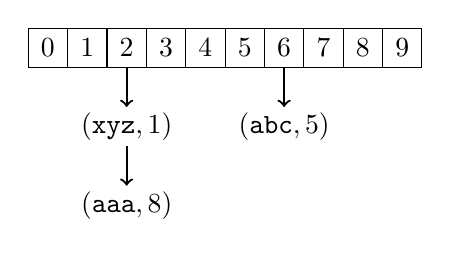
\begin{tikzpicture}[scale=0.5]
\draw (0,0) grid (10,1);
\foreach \x in {0,1,...,9} \node at (0.5+\x,0.5) {\x};
\draw[->,thick] (2.5,0) -- (2.5,-1);
\draw[->,thick] (6.5,0) -- (6.5,-1);
\draw[->,thick] (2.5,-2) -- (2.5,-3);
\node at (2.5,-3.5) {$(\texttt{aaa},8)$};
\node at (2.5,-1.5) {$(\texttt{xyz},1)$};
\node at (6.5,-1.5) {$(\texttt{abc},5)$};
\end{tikzpicture}
\caption{Hakemiston tallentaminen hajautustauluun.}
\label{fig:hajhak}
\end{figure}

Voimme myös toteuttaa hakemiston, jonka avaimet ovat kokonaislukuja.
Tällaisessa tietorakenteessa on järkeä, jos avaimet ovat niin suuria,
että emme voi käyttää sen sijasta tavallista taulukkoa.
Kuitenkin jos avaimet ovat pieniä kokonaislukuja,
taulukko on paljon parempi valinta, koska sen vakiokertoimet
ovat huomattavasti hajautustaulua pienemmät.

\section{Javan toteutukset}

Javassa on kaksi hajautustaulua käyttävää tietorakennetta:
\texttt{HashSet} pitää yllä alkioiden joukkoa
ja \texttt{HashMap} toteuttaa
hakemiston, jossa on avain-arvo-pareja.
Kummankin rakenteen operaatiot toimivat ajassa $O(1)$.

\subsection{\texttt{HashSet}-rakenne}

\texttt{HashSet} on alkioiden joukko,
johon voi lisätä alkion metodilla \texttt{add}
ja josta voi poistaa alkion metodilla \texttt{remove}.
Esimerkiksi seuraava koodi luo joukon, jossa voi olla
kokonaislukuja, ja lisää siihen luvut 3, 5 ja 8.
Tämän jälkeen koodi poistaa luvun 5 joukosta.

\begin{code}
HashSet<Integer> joukko = new HashSet<>();
joukko.add(3);
joukko.add(5);
joukko.add(8);
System.out.println(joukko); // [3, 5, 8]
joukko.remove(5);
System.out.println(joukko); // [3, 8]
\end{code}

Metodi \texttt{contains} kertoo, esiintyykö tietty alkio $x$ joukossa:

\begin{code}
if (joukko.contains(x)) {
    System.out.println("alkio on joukossa");
} else {
    System.out.println("alkiota ei ole joukossa");
}
\end{code}

Huomaa, että jokainen alkio voi esiintyä vain kerran joukossa.
Esimerkiksi vaikka seuraava koodi lisää luvun 5 kolmesti
joukkoon, se menee sinne vain ensimmäisellä kerralla ja
muut lisäykset jätetään huomiotta.

\begin{code}
HashSet<Integer> joukko = new HashSet<>();
joukko.add(5);
joukko.add(5);
joukko.add(5);
System.out.println(joukko); // [5]
\end{code}

\subsection{\texttt{HashMap}-rakenne}

\texttt{HashMap} luo hakemiston,
jossa on avain-arvo-pareja.
Hakemiston määrit\-telyssä tulee antaa
avaimen ja arvon tyyppi.
Metodi \texttt{put} lisää uuden avain-arvo-parin,
ja metodi \texttt{get} hakee arvon avaimen perusteella.

Esimerkiksi seuraava koodi luo sanakirjan, jossa sekä
avaimet että arvot ovat merkkijonoja.
Syötämme sanakirjaan merkkijonopareja, jotka kertovat
sanan käännöksen suomesta englanniksi.

\begin{code}
HashMap<String,String> sanakirja = new HashMap<>();

sanakirja.put("apina","monkey");
sanakirja.put("banaani","banana");
sanakirja.put("cembalo","harpsichord");

System.out.println(sanakirja.get("banaani")); // banana
\end{code}

Hyödyllinen on myös metodi \texttt{containsKey},
jonka avulla voi tarkastaa, onko tietylle avaimelle
tallennettu arvoa:

\begin{code}
if (sanakirja.containsKey(sana)) {
    System.out.println(sanakirja.get(sana));
} else {
    System.out.println("Sana puuttuu sanakirjasta!");
}
\end{code}

\subsection{Omat luokat}

Javan luokissa on metodi \texttt{hashCode},
jonka avulla olio kertoo pyydettäessä hajautusarvonsa.
Voimme esimerkiksi selvittää merkkijonon \texttt{apina}
hajautusarvon seuraavasti:

\begin{code}
System.out.println("apina".hashCode());
\end{code}

Tämä koodi tulostaa luvun 93022541,
joka on siis merkkijonon \texttt{apina} hajautusarvo Javassa.
On tunnettua, että Java käyttää merkkijonon hajautusarvon laskemiseen
polynomista hajautusta vakiolla $A=31$,
joten voimme laskea Javan hajautusarvon myös itse kaavalla
\[31^4 \cdot 97+31^3 \cdot 112+31^2 \cdot 105+31^1 \cdot 110+31^0 \cdot 97=93022541.\]

Jos haluamme käyttää omia olioitamme hajautustauluissa,
meidän täytyy toteuttaa luokkaan kaksi metodia:
\texttt{hashCode}, joka antaa olion hajautusarvon,
sekä \texttt{equals},
joka ilmaisee, ovatko kaksi oliota samat.
Metodi \texttt{hashCode} riittää toteuttaa niin,
että se palauttaa jonkin kokonaisluvun.
Metodi \texttt{equals} on tarpeen,
jotta Java pystyy varmistamaan, ovatko saman hajautusarvon
antavat oliot todella samat.

\section{Hajautustaulun käyttäminen}

Hajautustaulun ansiosta voimme käyttää algoritmeissamme
joukkoja ja hakemistoja, joiden operaatiot toimivat tehokkaasti.
Voimme alkajaisiksi ratkoa mukavammin ajassa $O(n)$ sellaisia ongelmia,
jotka olemme ratkoneet aiemmin järjestämisen avulla ajassa $O(n \log n)$.

Aloitamme ongelmasta, jossa haluamme selvittää,
montako eri alkiota taulukko sisältää.
Luvussa \ref{sec:taukas} ratkaisimme ongelman
järjestämällä taulukon ja tutkimalla sen jälkeen
vierekkäisiä alkioita.
Nyt kun käytös\-sämme on hajautustaulu, voimme vain lisätä
kaikki alkiot joukkoon ja hakea lopuksi joukon koon.
Näin saamme aikaan seuraavan algoritmin:

\begin{code}
alkiot = []
for i = 0 to n-1
    alkiot.add(taulu[i])
print(alkiot.size())
\end{code}

Tässä \texttt{alkiot} on hajautustaulua käyttävä joukko,
minkä ansiosta algoritmi toimii ajassa $O(n)$.

Tarkastellaan sitten ongelmaa, jossa haluamme selvittää
taulukon yleisimmän alkion.
Ratkaisimme tämänkin ongelman aiemmin
järjestä\-mällä taulukon, mutta
hajautustaulun avulla voimme lähestyä ongelmaa
toisella tavalla luomalla hakemiston,
jonka avaimet ovat taulukon alkioita ja arvot niiden
esiintymiskertoja.
Nyt voimme vain käydä läpi taulukon sisällön ja
pitää kirjaa, montako kertaa mikäkin alkio esiintyy taulukossa:

\begin{code}
laskuri = []
suurin = 0
for i = 0 to n-1
    laskuri[taulu[i]]++
    if laskuri[taulu[i]] > suurin
        suurin = laskuri[taulu[i]]
        yleisin = taulu[i]
print(yleisin)
\end{code}

Tässä hakemisto \texttt{laskuri}
on toteutettu hajautustaulun avulla,
jolloin avaimet voivat olla mitä tahansa lukuja
ja operaatiot toimivat ajassa $O(1)$.
Tuloksena on algoritmi, jonka aikavaativuus on $O(n)$.

Kuten nämä esimerkit osoittavat, hajautustaulu
\emph{helpottaa} algoritmien luomista,
koska meidän ei tarvitse pukea ongelmia järjestämisen muotoon
vaan voimme käsitellä niitä suoremmin.
Mutta toisaalta olemme ratkoneet vain uudestaan tehtäviä,
jotka ovat hoituneet mainiosti myös järjestämisen avulla.
Antaisiko hajautustaulu meille jotain todellisia uusia
mahdollisuuksia algoritmien suunnittelussa?

Hajautustaulu osoittaa todelliset kyntensä silloin,
kun haluamme pitää yllä aidosti \emph{dynaamista}
tietorakennetta eli haluamme vuorotellen muuttaa
tietorakennetta ja hakea sieltä tietoa.
Tällöin emme voi enää toteuttaa algoritmia,
joka järjestää koko aineiston kerran alussa.
Esimerkki tällaisesta tehtävästä on,
että käytössämme on funktio \texttt{haeLuku},
joka antaa lukuja yksi kerrallaan.
Jokaisen luvun jälkeen meidän tulee ilmoittaa,
montako eri lukua olemme saaneet tähän mennessä,
ennen kuin voimme pyytää funktiolta seuraavan luvun.
Voimme ratkaista tehtävän seuraavasti ajassa $O(n)$
hajautustaulun avulla:

\begin{code}
alkiot = []
for i = 1 to n
    luku = haeLuku()
    alkiot.add(luku)
    print(alkiot.size())
\end{code}

\index{online-algoritmi}
\index{offline-algoritmi}

Tällaisesta algoritmista käytetään joskus nimeä
\emph{online-algoritmi}.
Tämä tarkoittaa, että algoritmille annetaan syötettä
alkio kerrallaan ja algoritmi pystyy ilmoittamaan senhetkisen
vastauksen joka alkion käsittelyn jälkeen.
Vastaavasti \emph{offline-algoritmi} tarvitsee
käyttöönsä heti koko syötteen,
jotta se voi käsitellä syötettä kokonaisuutena,
kuten järjestää sen.
Monissa tehtävissä online-algoritmi on vaikeampi
keksiä kuin offline-algoritmi.
